\documentclass[12pt,a4paper]{article}

\usepackage{indentfirst}
\usepackage{amssymb}
\usepackage{graphicx}
\usepackage{longtable}
\usepackage{fancyhdr}
\usepackage{booktabs}  
\usepackage{xeCJK}
\usepackage{enumerate}
\usepackage{geometry}
\usepackage{array}

\geometry{left=2cm,right=2cm,top=3cm,bottom=3cm}
\setmainfont{LiHei Pro}
\setmonofont{Helvetica}
\setCJKmainfont[ItalicFont={Heiti TC Light}, BoldFont={LiHei Pro}]{Heiti TC Light}
\pagestyle{fancy}
\XeTeXlinebreakskip = 0pt plus 1pt
%設定段落之間的距離
\setlength{\parskip}{0cm}
%設定行距
\linespread{1.2}\selectfont

\lhead{2017年國際資訊奧林匹亞}
\rhead{立人高中校內排名賽}

\begin{document}

{\LARGE \textbf{\begin{center}台中市私立立人高級中學 \\ 程式設計校內排名賽\end{center}}}

\begin{center}\framebox{\begin{minipage}{\textwidth}{

{\LARGE \textbf{\begin{center}作答說明\end{center}}}

\begin{itemize}
\item 比賽時間為 2016/08/20 早上 9 點到下午 1 點,確切時間以評分系統為準。
\item 可使用C / C++ / Python 語言作答。
\item 本次共有6道試題,滿分 100 分。每題中各測試資料配分以評測系統為主。
\item long long int 型態於 scanf, printf 中請使用 \%lld。
\item 除了第五題須每隔 180 秒才能上傳一次外,其餘題目皆需 75 秒才能再度上傳。
\end{itemize}
~\\
}\end{minipage}}\end{center}

\begin{table}[h]
\centering
\begin{tabular}{ccccc}
\toprule[1.5pt]
~&\textbf{題目名稱}&\textbf{占分}&\textbf{執行時間限制}&\textbf{記憶體限制}\\
\midrule[1.5pt]
第1題&A4&16&0.5 秒&128 MiB\\
\midrule[0.75pt]
第2題&A10&16&0.5 秒&128 MiB\\
\midrule[0.75pt]
第3題&A53&17&0.5 秒&128 MiB\\
\midrule[0.75pt]
第4題&A9&17&1.0 秒&128 MiB\\
\midrule[0.75pt]
第5題&A3&17&1.0 秒&128 MiB\\
\midrule[0.75pt]
第6題&ATP&17&1.0 秒&128 MiB\\
\bottomrule[1.5pt]
\end{tabular} 
\end{table}


\newpage

\begin{center}
\textbf{{\Huge 第1題\\A4\\}~\\執行時間限制: 0.5 秒\\記憶體限制: 128 MiB}
\end{center}


\subsection*{$\blacksquare$題目敘述}

一年一度的高中摺紙季又到了!在摺紙季中,所有同學都會試著把他們手上的考卷一直對折、一直對折,一直對折到這一個紙張的長、寬皆不大於 $1$ 為止,然後我們稱最後摺完的成品稱作一張合格的作品。因為考卷可能很大張、可能很小張,所以在摺紙季的時候,每個同學都需要絞盡腦汁來想:我要怎麼樣才能將一張考卷,用最快的速度,每次只能對摺,對摺到合格為止?

\begin{center}
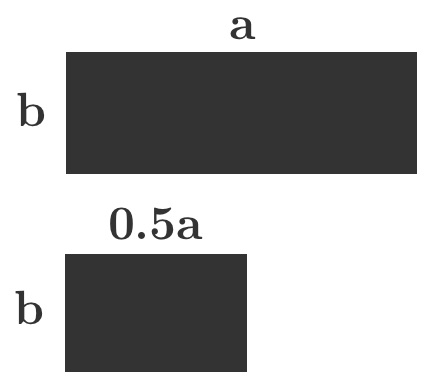
\includegraphics[scale=0.5]{1-1.jpg}
\end{center}

上圖是簡單的示意圖,當一張長寬為 $(a, b)$ 的考卷沿著 $a$ 邊對折一半之後,其長寬變成 $(a/2, b)$。當然你也可以沿著 $b$ 邊來摺。

今天給你一張長寬分別為 $(a, b)$ 的考卷,請問至少需要對摺幾次才能使得所有邊長皆不大於 $1$?

\subsection*{$\blacksquare$輸入說明}
每組測試資料包含一行。\par
第一行包含兩個正整數\(a,b\),分別以一個空白間隔。\par

\subsection*{$\blacksquare$輸出說明}
印出一行,包含一個數字,該數字即為最少的對摺次數。\\

\subsection*{$\blacksquare$輸入範圍限制}
\(0 < a, b \leq 10^{17} \) \par



\subsection*{$\blacksquare$子問題}
\begin{table}[h]
\centering
\begin{tabular}{ccll}
\toprule[1.5pt]
\textbf{子任務}&\textbf{分數}&\multicolumn{1}{c}{\textbf{額外輸入限制}}&\multicolumn{1}{c}{\textbf{滿足此子任務的範例測資}}\\
\midrule[1.5pt]
1&2& $a, b \leq  10^3 $ &1, 2\\
\midrule[0.75pt]
2&3& $a, b \in S, S = \{2^k \mid k \in \mathbb{N} \}$ &2\\
\midrule[0.75pt]
3&11& 無額外限制&1, 2\\
\bottomrule[1.5pt]
\end{tabular}
\end{table}


\subsection*{$\blacksquare$範例測試 1}
\begin{tabular}{cc}
輸入資料&輸出資料\\ 
\framebox{\begin{minipage}{0.45\linewidth}
\texttt{3 2\\}
\end{minipage}}
&
\framebox{\begin{minipage}{0.45\linewidth}
\texttt{3\\
}\end{minipage}}\\ 
\end{tabular}

\subsection*{$\blacksquare$範例測試 2}
\begin{tabular}{cc}
輸入資料&輸出資料\\ 
\framebox{\begin{minipage}{0.45\linewidth}
\texttt{137438953472 18014398509481984\\}
\end{minipage}}
&
\framebox{\begin{minipage}{0.45\linewidth}
\texttt{91\\
}\end{minipage}}\\ 
\end{tabular}

\newpage

\begin{center}
\textbf{{\Huge 第2題\\A10\\}~\\執行時間限制: 0.5 秒\\記憶體限制: 128 MiB}
\end{center}


\subsection*{$\blacksquare$題目敘述}

「傳紙條啊傳紙條!」校園內張貼起了一張海報,印著這樣的標語。

這時在電腦教室內打計算幾何的諺諺想到了一個問題:「如果我有 $n$ 張不同長度的紙條(寬度都一樣),接著我恰好在這些紙條上面任意拿剪刀剪 $k$ 刀(只能垂直長邊下去剪),那在剪完之後所有紙條的最小值,最大可能為多少?」

\begin{center}
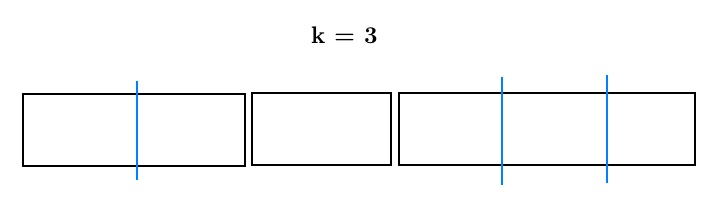
\includegraphics[scale=0.5]{2-1.jpg}
\end{center}

上圖是簡單的示意圖,有 $n = 3$張不同長度的紙條,現在我們一定要對他切 $k = 3$ 刀。現在我們要求的就是,去計算每一個切完後的紙條,取最小值,請問這個最小值的最大可能為多少?

為了計算方便,我們限制對於每一個紙條(包含切之後的產生的紙條),當切了一刀,剩下的兩個紙條都必須為正整數長度。

\subsection*{$\blacksquare$輸入說明}
每組測試資料包含兩行。\par
第一行包含兩個整數\(n,k\),分別以一個空白間隔。\par
第二行有 $n$ 個正整數 $l_1, l_2, ... l_n$,表示在還沒切時,每個紙條的長度,分別以一個空白分隔。\par

\subsection*{$\blacksquare$輸出說明}
印出一行,包含一個數字,該數字即為在切 $k$ 刀的情況下,其最終每個紙條的最小值的最大可能的值。\par

\subsection*{$\blacksquare$輸入範圍限制}
\(1 \leq n \leq 10^{5} \) \par
\(0 \leq k \leq 10^{5} \) \par
\(1 \leq l_i \leq 10^{9} \) \par
\( k \leq \sum (l_i-1) \) \par



\subsection*{$\blacksquare$子問題}
\begin{table}[h]
\centering
\begin{tabular}{ccll}
\toprule[1.5pt]
\textbf{子任務}&\textbf{分數}&\multicolumn{1}{c}{\textbf{額外輸入限制}}&\multicolumn{1}{c}{\textbf{滿足此子任務的範例測資}}\\
\midrule[1.5pt]
1&2& $n, k \leq 12 $ &1, 2\\
\midrule[0.75pt]
2&4& $n \leq 10^3, l_i \leq 10^3$ &1\\
\midrule[0.75pt]
3&10& 無額外限制&1, 2\\
\bottomrule[1.5pt]
\end{tabular}
\end{table}


\subsection*{$\blacksquare$範例測試 1}
\begin{tabular}{cc}
輸入資料&輸出資料\\ 
\framebox{\begin{minipage}{0.45\linewidth}
\texttt{5 3\\
189 162 240 170 210\\}
\end{minipage}}
&
\framebox{\begin{minipage}{0.45\linewidth}
\texttt{94\\
}\end{minipage}}\\ 
\end{tabular}
  
  
 \\

範例測試 1 說明了:我們或許可以選擇切長度為 $189$ 的紙條成兩張,分別為 $94, 95$;切長度 $240$ 為 $120, 120$;切長度 $210$ 為 $105, 105$。 此時全部的紙條最短為 $94$,而這種切法可以讓最短的那張紙條,長度最長。\par


\subsection*{$\blacksquare$範例測試 2}
\begin{tabular}{cc}
輸入資料&輸出資料\\ 
\framebox{\begin{minipage}{0.45\linewidth}
\texttt{12 2\\
388 46 436 235 341 278 161 352 2 268 372 334\\
}
\end{minipage}}
&
\framebox{\begin{minipage}{0.45\linewidth}
\texttt{2\\
}\end{minipage}}\\ 
\end{tabular}

\newpage

\begin{center}
\textbf{{\Huge 第3題\\A53\\}~\\執行時間限制: 0.5 秒\\記憶體限制: 128 MiB}
\end{center}


\subsection*{$\blacksquare$題目敘述}

「跳格子啊跳格子!」校園內張貼起了一張海報,印著這樣的標語。

從小就喜歡跳格子的覺得跳格子真的是非常的有趣,於是他打算去改良原本的跳格子遊戲,變成進階版的「跳矩陣遊戲」。這個遊戲是由一個 $n$ (row)乘以 $m$ (column)的格子所組成,每個格子可能有紅、綠、藍(編號為 $0, 1, 2$)三種顏色。\par

\begin{center}
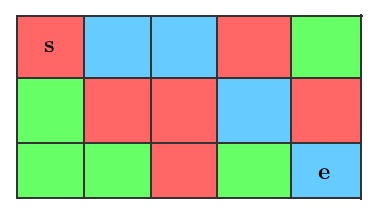
\includegraphics[scale=0.5]{3-1.jpg}
\\
格子可能有三種顏色,總共有 $n*m$ 個格子。
\end{center}

這個遊戲的規則是需要玩家從最左上角的格子,一直跳到最右下角的格子。跳的規格是每次可以往右、下、右下三個方位去跳,而最後我們需要計算到達終點時的總積分,這個積分的計算方式為:從起點開始,每次從格子 $A$(格子 $A$ 的顏色為編號 $a$) 跳到格子 $B$(格子 $B$ 的顏色為編號 $b$),需要加上一個給定的數值為 $C_{ab}$。\par

給定數值方陣 $C$,矩陣的長寬與顏色資訊(紅色為 $0$,綠色為 $1$,藍色為 $2$),請問到達終點時,最大的總積分為多少?\par

\subsection*{$\blacksquare$輸入說明}
每組測試資料包含很多行。\par
第一行包含兩個正整數\(n,m\),分別以一個空白間隔。\par
接下來有一個數值方陣,共三行($i = 0, 1, 2$),每行有 $3$ 個正整數 $C_{i0}, C_{i1}, C_{i2}$,表示數值方陣 $C$ 的數值,分別以一個空白間隔。\par
接下來有 $n$ 行,每行有 $m$ 個數字,表示每個格子的顏色編號 $A_{ij} $(紅色為 $0$,綠色為 $1$,藍色為 $2$),其之間以一個空白分開。

\subsection*{$\blacksquare$輸出說明}
印出一行,包含一個數字,該數字到達右下角終點時,最大的總積分。\par

\subsection*{$\blacksquare$輸入範圍限制}
\(n, m \leq 1000 \) \par
\(A_{ij} \in \{0, 1, 2\} \) \par
\(1 \leq C_{ij} \leq 10^{6} \) ,且保證 $C_{ij} = C{ji}$ \par 



\subsection*{$\blacksquare$子問題}
\begin{table}[h]
\centering
\begin{tabular}{ccll}
\toprule[1.5pt]
\textbf{子任務}&\textbf{分數}&\multicolumn{1}{c}{\textbf{額外輸入限制}}&\multicolumn{1}{c}{\textbf{滿足此子任務的範例測資}}\\
\midrule[1.5pt]
1&4& $n \leq 5 $ &1, 2\\
\midrule[0.75pt]
2&5& $n \leq 100 $ &1, 2\\
\midrule[0.75pt]
3&8& 無額外限制&1, 2\\
\bottomrule[1.5pt]
\end{tabular}
\end{table}


\subsection*{$\blacksquare$範例測試 1}
\begin{tabular}{cc}
輸入資料&輸出資料\\ 
\framebox{\begin{minipage}{0.45\linewidth}
\texttt{2 2\\
3 7 2\\
7 4 3\\
2 3 1\\
0 1\\
2 0\\
}
\end{minipage}}
&
\framebox{\begin{minipage}{0.45\linewidth}
\texttt{14\\
}\end{minipage}}\\ 
\end{tabular}

 \\

對於範例測試 1,我們可以選擇從 $(0, 0)$ 走到 $(0, 1)$(積分 $+7$),再從 $(0, 1)$ 走到 $(1, 1)$(積分 $+7$),總積分為 14 會是此輸入中最大的。\\

請注意輸入格式。\\

\newpage

\begin{center}
\textbf{{\Huge 第4題\\A9\\}~\\執行時間限制: 1.0 秒\\記憶體限制: 128 MiB}
\end{center}


\subsection*{$\blacksquare$題目敘述}

「九連環!九連環!九連環完再來玩!」校園內張貼起了一張海報,印著這樣的標語。\\

九連環實際上是一個中國傳統的智力遊戲,這一個遊戲實際上由九個圈圈和一把劍組成。安安是一個愛玩遊戲的女生,他喜歡挑戰各種不同的遊戲,像是剪刀石頭布、黑白猜、竹筍、海帶阿海帶等等遊戲。有一天他看到了海報。他很好奇,馬上去問問學校裡面最資深的國學老師。想當然爾,他馬上就開始透過老師的介紹,嘗試玩這款智力遊戲!\\

這一個九連環遊戲由九個環和一把劍組成,而我們的目標是將劍上的這九個環全部取下來,也就是把劍和環都分開。這個遊戲的規則很特別,因為要實際玩過才有辦法想像整個遊戲的運作過程,在這裡就不附上圖;但我們可以用簡單的幾個描述,來完整的敘述整個遊戲過程:\\

假想一開始所有環都套在劍的上面,假設總共有 $n$ 個環,編號 $1, 2, .... n$,套到劍裡面。請參照下述規則進行遊戲。這時候我們可以做兩種操作:\\

\begin{itemize}
\item 1. 編號為 1 的環可以隨時取下,也可以直接掛上。
\item 2. 如果編號為 $1.... k-1$ 的環都已經拿下來了,而且編號 $k$ 的環還在劍上,那麼隨時可以取下或掛上編號 $k+1$ 的環。
\end{itemize}

今天給你一個 $n$ 連環,請問他「最少」需要做多少次操作才能將全部的環取下來?

如果輸入的 $n \leq 10$,請按照操作順序,輸出所有操作方案。格式請見範例輸入 $1, 3$。

\subsection*{$\blacksquare$輸入說明}
每組測試資料只有一行。\par
第一行有個正整數\(n\),表示這是一個 $n$ 連環的問題。\par

\subsection*{$\blacksquare$輸出說明}
如果 $n \leq 10$,請輸出操作的總次數並換行後,再輸出每一個操作,可能是 "Move ring (環的編號) in/out",每個操作後請換行。\par
如果 $n > 10$,請只輸出一個數字,表示操作的總次數。如果這個數字太大,請模 $1, 000, 000, 007$ 再輸出。

\subsection*{$\blacksquare$輸入範圍限制}
\(n \leq 10^{17} \) \par


\subsection*{$\blacksquare$子問題}
\begin{table}[h]
\centering
\begin{tabular}{ccll}
\toprule[1.5pt]
\textbf{子任務}&\textbf{分數}&\multicolumn{1}{c}{\textbf{額外輸入限制}}&\multicolumn{1}{c}{\textbf{滿足此子任務的範例測資}}\\
\midrule[1.5pt]
1&7& $n \leq 10 $ &1, 3\\
\midrule[0.75pt]
2&7& $ 11 \leq n \leq 10^6 $ &2\\
\midrule[0.75pt]
3&3& $ 11 \leq n $ &2\\
\bottomrule[1.5pt]
\end{tabular}
\end{table}


\subsection*{$\blacksquare$範例測試 1}
\begin{tabular}{cc}
輸入資料&輸出資料\\ 
\framebox{\begin{minipage}{0.45\linewidth}
\texttt{3
}
\end{minipage}}
&
\framebox{\begin{minipage}{0.45\linewidth}
\texttt{5\\
Move ring 1 out\\
Move ring 3 out\\
Move ring 1 in\\
Move ring 2 out\\
Move ring 1 out\\
}\end{minipage}}\\ 
\end{tabular}

\subsection*{$\blacksquare$範例測試 2}
\begin{tabular}{cc}
輸入資料&輸出資料\\ 
\framebox{\begin{minipage}{0.45\linewidth}
\texttt{678679\\
}
\end{minipage}}
&
\framebox{\begin{minipage}{0.45\linewidth}
\texttt{274251827\\
}\end{minipage}}\\ 
\end{tabular}

\subsection*{$\blacksquare$範例測試 3}
\begin{tabular}{cc}
輸入資料&輸出資料\\ 
\framebox{\begin{minipage}{0.45\linewidth}
\texttt{5\\
}
\end{minipage}}
&
\framebox{\begin{minipage}{0.45\linewidth}
\texttt{21\\
Move ring 1 out\\
Move ring 3 out\\
Move ring 1 in\\
Move ring 2 out\\
Move ring 1 out\\
Move ring 5 out\\
Move ring 1 in\\
Move ring 2 in\\
Move ring 1 out\\
Move ring 3 in\\
Move ring 1 in\\
Move ring 2 out\\
Move ring 1 out\\
Move ring 4 out\\
Move ring 1 in\\
Move ring 2 in\\
Move ring 1 out\\
Move ring 3 out\\
Move ring 1 in\\
Move ring 2 out\\
Move ring 1 out\\
}\end{minipage}}\\ 
\end{tabular}


\newpage


\begin{center}
\textbf{{\Huge 第5題\\A3 (Special Judge)\\}~\\執行時間限制: 1.0 秒\\記憶體限制: 128 MiB}
\end{center}


\subsection*{$\blacksquare$題目敘述}

「不要模仿我!」校園內張貼起了一張海報,印著這樣的標語。\\

據說是因為實在太多調皮搗蛋的學生喜歡亂模仿別人的動作,於是教官室想到了一個對策:如果一個學生模仿別人的動作,他就會被叫去教官室;這時候教官會給他一個題目,請他來回答。如果這位學生答對,那麼他就可以不用被記過,反之亦然。\\

這一個問題是這樣子的,今天教官給你 $n$ 種大寫字母的卡片,每種都有無限多張。你需要從這 $n$ 種都是無限多張的字卡裡面,挑出 $L$ 張出來排成一列字串。教官希望你可以不要再模仿別人,所以學生必須找出一種排列方法,使得「對於所有的連續區間皆不相同」,比方說:假設今天有三種大寫字母,分別是 $A, B, C$,那我們可以組成 $ABAC$, $BABC$, $CABC$, $ACBA$ 等等都滿足條件;而 $ABAB$ 不符合條件,因為 $AB$ 連續出現了兩次;$CABCABCA$ 也不符合條件,因為有連續的 $ABC$ 和連續的 $CAB$。\\

今天有一個學生被叫到教官室去回答這個問題,因為他覺得很難,想請你寫一個程式解決!\\

今給定 $n$ 種卡片,請你輸出一個符合條件的字串,系統將依據你所輸出的符合條件之字串「長度」做評分。

\subsection*{$\blacksquare$輸入說明}
每組測試資料只有一行。\par
第一行有個正整數\(n\),表示總共有 $n$ 種字母(這些字母由 $A, B, C, D, ...$ 以此類推,如果 $n = 6$,那將有 $A, B, C, D, E, F$ 六種字母),各有無限多個。\par

\subsection*{$\blacksquare$輸出說明}
請輸出一行,包含一個字串,表示符合教官問題條件的字串。這個字串的長度最少為 0,最多只能輸出 $10^5$ 個字元。評分方式會依照你的字串長度做評分,越長的字串分數越高。得分計算公式:假設你輸出的符合條件之字串長度為 $S$,\\

則得分為 $0.1*(\frac{S}{10^5})^{0.2} * (該筆 subtask 分數)$,(若 $S = 10^5$,則得到該 Subtask 全部分數)。

\subsection*{$\blacksquare$輸入範圍限制}
\( n \in \{3, 12, 20\} \) \par


\subsection*{$\blacksquare$子問題}
\begin{table}[h]
\centering
\begin{tabular}{ccll}
\toprule[1.5pt]
\textbf{子任務}&\textbf{分數}&\multicolumn{1}{c}{\textbf{額外輸入限制}}&\multicolumn{1}{c}{\textbf{滿足此子任務的範例測資}}\\
\midrule[1.5pt]
1&5& $n = 20 $ &1\\
\midrule[0.75pt]
2&5& $n = 12 $ &無\\
\midrule[0.75pt]
3&7& $n = 3 $ &無\\
\bottomrule[1.5pt]
\end{tabular}
\end{table}


\subsection*{$\blacksquare$範例測試 1}
\begin{tabular}{cc}
輸入資料&輸出資料\\ 
\framebox{\begin{minipage}{0.45\linewidth}
\texttt{20
}
\end{minipage}}
&
\framebox{\begin{minipage}{0.45\linewidth}
\texttt{ABCDEFGHIJKLMNOPQRST
}\end{minipage}}\\ 
\end{tabular}

 \\

此筆輸出的得分為 $0.91$ 分。

\subsection*{$\blacksquare$範例測試 2}
\begin{tabular}{cc}
輸入資料&輸出資料\\ 
\framebox{\begin{minipage}{0.45\linewidth}
\texttt{20
}
\end{minipage}}
&
\framebox{\begin{minipage}{0.45\linewidth}
\texttt{ABCDEFGHIJKLMNOPQRSTABCDEFG\\HIJKLMNOPQRST
}\end{minipage}}\\ 
\end{tabular}

 \\

此筆輸出的得分為 $0$ 分,違反教官的條件,你要被教官痛扁一頓了!

\newpage

\begin{center}
\textbf{{\Huge 第6題\\ATP\\}~\\執行時間限制: 1.0 秒\\記憶體限制: 128 MiB}
\end{center}


\subsection*{$\blacksquare$題目敘述}

「將頭髮梳成大人模樣,穿上一身帥氣西裝。」校園內張貼起了一張海報,印著這樣的標語。\\

不知道你還記不記得那些年電影的畫面呢?青春總是特別令人回味不已啊!尤其是海邊。在海邊,總是可以帶給人特別的回憶、更多的不一樣。於是即將畢業的樂樂同學,找了一些朋友一起到海邊去,希望回味青春奔放的美好。樂樂這一群人總共有 $n$ 個人,他們決定坐在堤防上談天說笑,便由左到右坐成一排(由左到右,分別編號 $1 ...... n $),坐在堤防上。\\

特別的是,因為樂樂一群人很特別,每個人的頭不是朝向左邊(left)看就是朝向右邊(right)看。假設編號為 $k$ 的的朝左邊看,那們他可以看到編號 $1$ 到編號 $k-1$ 之間所有人的狀況;若朝右邊,他他可以看到編號 $k+1$ 到 $n$ 所有人的狀況。\\

小智就住在海岸旁邊,每次看到這種想回味青春的學生總是會來惡作劇一番。小智打算對正坐在岸上的樂樂這 $n$ 個人這群下手。他打算在每個人的頭上都放上恰好一隻毛毛蟲,而放的方式就是放完一個人的、再放另外一個人。 只要一個人的頭上被放了毛毛蟲,他就會暈倒,不會再看到別人的狀況。\\

樂樂和他的朋友其實都很愛哭。還沒暈倒的每個人,只要看到他的朋友的頭上被放一隻毛毛蟲,他就會掉下一滴眼淚來。\\

小智只是想惡作劇,但他也不想傷害人。所以他希望讓大家所掉的眼淚滴數總和越少越好,但是又能夠在每個人頭上都放一隻毛毛蟲,所以你需要決定放毛毛蟲的順序。請問,要完成小智的任務,最少會讓這 $n$ 個人總共掉多少滴眼淚?\\



\subsection*{$\blacksquare$輸入說明}
每組測試資料包含兩行。\par
第一行包含一個整數 $n$,表示總共有 $n$ 個人(包含樂樂)。\par
第二行有一個字串 $S$,從左到右第 $k$ 個字元 $S_k$ 如果為 "R",表示編號為 $k$ 的同學頭朝向右邊看;如果為 "L",就是朝向左邊看。\par

\subsection*{$\blacksquare$輸出說明}
請只輸出一個整數,表示滿足小智的任務下,最少會讓這 $n$ 個人總共掉多少眼淚。\par

\subsection*{$\blacksquare$輸入範圍限制}
\( 1 \leq n \leq 1 000 000 \) \par


\subsection*{$\blacksquare$子問題}
\begin{table}[h]
\centering
\begin{tabular}{ccll}
\toprule[1.5pt]
\textbf{子任務}&\textbf{分數}&\multicolumn{1}{c}{\textbf{額外輸入限制}}&\multicolumn{1}{c}{\textbf{滿足此子任務的範例測資}}\\
\midrule[1.5pt]
1&1& $n \leq 5 $ &1, 2\\
\midrule[0.75pt]
2&2& $n \leq 12 $ &1, 2\\
\midrule[0.75pt]
3&3& $n \leq 1000 $ &1, 2\\
\midrule[0.75pt]
4&11& 沒有額外限制&1, 2\\
\bottomrule[1.5pt]
\end{tabular}
\end{table}


\subsection*{$\blacksquare$範例測試 1}
\begin{tabular}{cc}
輸入資料&輸出資料\\ 
\framebox{\begin{minipage}{0.45\linewidth}
\texttt{5\\
LRLRR
}
\end{minipage}}
&
\framebox{\begin{minipage}{0.45\linewidth}
\texttt{1
}\end{minipage}}\\ 
\end{tabular}




\newpage

\end{document}
